\documentclass[12pt,spanish]{article}
\usepackage[spanish]{babel}
\usepackage{graphicx}
\usepackage{color}
\usepackage{xcolor}
\usepackage{colortbl}
\usepackage{amsthm,thmtools}
\usepackage{dirtytalk}
\usepackage{multirow}
\usepackage{amsmath}
\usepackage{subcaption}
\usepackage{adjustbox}
\usepackage{amsmath}
\usepackage{centernot}
\usepackage{mathtools}
\usepackage{multirow}
\usepackage[hidelinks]{hyperref}
\usepackage{caption}
\usepackage{eurosym} % para el euro
\usepackage{amsthm}
\usepackage{multicol}
\usepackage{float}
\usepackage{amsfonts}
\usepackage{titling}
\usepackage{soul}
\usepackage{listings}
\usepackage{listingsutf8}
\usepackage{array}
\usepackage{tikz}
\usetikzlibrary{shapes.geometric, arrows, chains, calc,positioning,fit,decorations.pathreplacing}
\usepackage[framemethod=tikz]{mdframed}

\graphicspath{ {../img/}}
\selectlanguage{spanish}
\usepackage[utf8]{inputenc}
\usepackage{graphicx}
\usepackage[a4paper,left=3cm,right=2cm,top=2.5cm,bottom=2.5cm]{geometry}

\newenvironment{solution}{
	\par
	\textbf{Solución}
	\par
	\begin{center}
}
{
	\end{center}
}

\lstset{
  breaklines=true,
  postbreak=\mbox{\textcolor{red}{$\hookrightarrow$}\space},
}


\title{Servidores Web de Altas Prestaciones}
\setlength{\droptitle}{10em}
\author{Carlos Sánchez Páez}

\makeindex
\begin{document}
\definecolor{light-gray}{gray}{0.95}
\lstset{columns=fullflexible,basicstyle=\ttfamily}
\surroundwithmdframed[
  hidealllines=true,
  backgroundcolor=light-gray,
  innerleftmargin=0pt,
  innertopmargin=0pt,
  innerbottommargin=0pt]{lstlisting}


\begin{titlepage}

 \newlength{\centeroffset}
 \setlength{\centeroffset}{-0.5\oddsidemargin}
 \addtolength{\centeroffset}{0.5\evensidemargin}
 \thispagestyle{empty}

 \noindent\hspace*{\centeroffset}
 \begin{minipage}{\textwidth}

  \centering
  
\includegraphics[width=0.9\textwidth]{logo_ugr.jpg}\\[1.4cm]

  \textsc{ \Large Servidores Web de Altas Prestaciones\\[0.2cm]}
  \textsc{GRADO EN INGENIERÍA INFORMÁTICA}\\[1cm]

  {\Huge\bfseries Prácticas resueltas \\}
 \end{minipage}

 \vspace{1.5cm}
 \noindent\hspace*{\centeroffset}
 \begin{minipage}{\textwidth}
  \centering

  \textbf{Autor}\\ {Carlos Sánchez Páez}\\[2.5ex]
  
\includegraphics[width=0.4\textwidth]{etsiit_logo.png}\\[0.1cm]
  \vspace{1.5cm}
  
\includegraphics[width=0.15\textwidth]{atc.jpg}\\[0.1cm]
  \vspace{1cm}
  \textsc{Escuela Técnica Superior de Ingenierías Informática y de Telecomunicación}\\
  \vspace{1cm}
  \textsc{Curso 2019-2020}
 \end{minipage}
\end{titlepage}
\thispagestyle{empty}
\newpage
\tableofcontents{}
\newpage

\section{Práctica 1}

En esta práctica configuraremos dos máquinas virtuales (\textit{M1} y \textit{M2}). También crearemos una interfaz \emph{host-only} para que las máquinas puedan conectarse entre ellas. \\

En esta guía configuraremos la interfaz sólo anfitrión manualmente en una máquina. En la otra dejaremos que el asistente de instalación lo haga por nosotros.

\begin{enumerate}
	\item Comenzaremos creando las máquinas virtuales desde VirtualBox. Las proveeremos de al menos 512MB de RAM y 10GB de disco duro.
	\item Descargamos la imagen ISO de Ubuntu Server 18.04 y la montamos en la unidad de disco de la primera máquina.
	\item Arrancamos la máquina e iniciamos el asistente de instalación. Establecemos nuestro nombre de usuario de GitHub como \emph{username} y \emph{m1} como nombre del servidor. La clave será \emph{Swap1234}
	\item Cuando termine la instalación apagamos la máquina.
	\item En VirtualBox abrimos el administrador de redes sólo antitrión (dentro del menú Archivo).
	\item Creamos un adaptador y activamos DHCP para que asigne una IP a nuestra máquina.
	\begin{figure}[H]
		\centering
		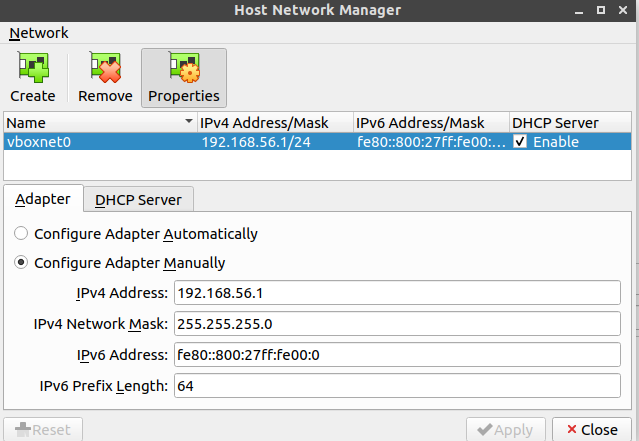
\includegraphics[scale=0.65]{/p1/host_only.png}
	\end{figure}
	\item Vamos a los ajustes de red de la máquina y ''conectamos'' el adaptador que acabamos de crear.
	\begin{figure}[H]
		\centering
		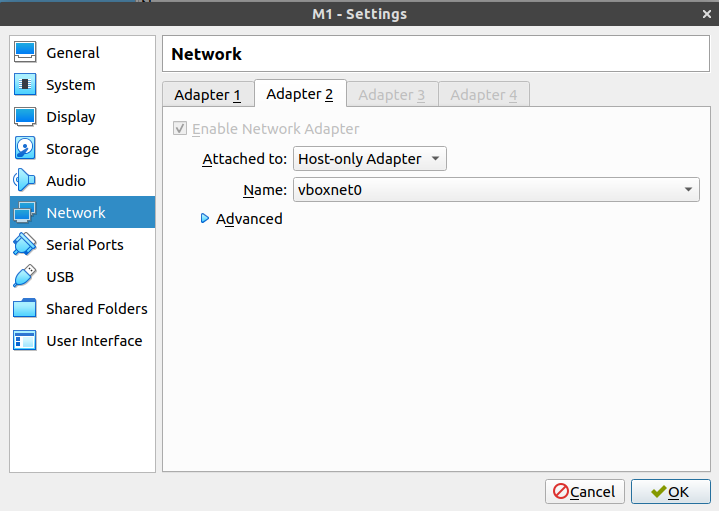
\includegraphics[scale=0.65]{/p1/host_only_2.png}
	\end{figure}
	\item Arrancamos la máquina. Ejecutamos el siguiente comando para ver las interfaces conectadas:
	\begin{lstlisting}
		m1> sudo ifconfig -a
	\end{lstlisting}
	\begin{figure}[H]
		\centering
		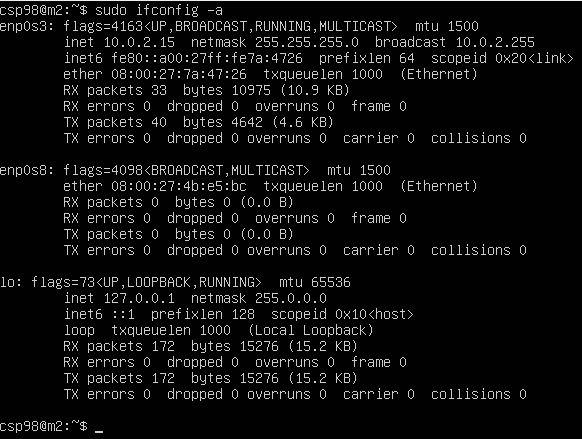
\includegraphics[scale=0.65]{/p1/ifconfig_noip.png}
	\end{figure}
	\item Vemos que tenemos una nueva interfaz (\emph{enp0s8}) pero no tiene IP asignada. Para arreglar esto usaremos \emph{netplan}.
	\item Creamos un archivo de configuración para ella:
	\begin{lstlisting}
		m1> sudo nano /etc/netplan/host-only.yaml
	\end{lstlisting}
	\item Introducimos este contenido en el archivo. Debemos usar espacios en vez de tabuladores.
	\begin{lstlisting}
		network:
		  version: 2
			renderer: networkd
			ethernets:
			  enp0s8:
				  dhcp4: true
	\end{lstlisting}
	\item Guardamos los cambios y los aplicamos con el comando
	\begin{lstlisting}
		m1> sudo netplan apply
	\end{lstlisting}
	\item Ejecutamos \emph{sudo ifconfig -a} y comprobamos que ya tenemos IP asignada:
	\begin{figure}[H]
		\centering
		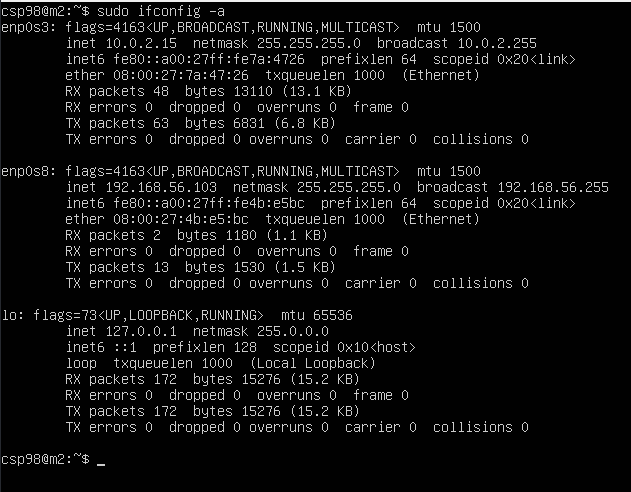
\includegraphics[scale=0.65]{/p1/ifconfig.png}
	\end{figure}
	\item Instalamos la pila LAMP:
	\begin{lstlisting}
	m1> sudo apt install -y openssh-server openssh-client apache2 mysql-server mysql-client
	\end{lstlisting}
	\item Pasamos ahora a la configuración de \emph{m2}. Para ello seguimos los pasos anteriores. Como el adaptador sólo anfitrión ya está creado, el asistente de instalación lo configurará automáticamente. Lo único que tenemos que hacer es ''conectarlo'' a la máquina como hicimos antes.
	\item Cuando termine la instalación, ejecutamos el comando anterior para instalar la pila LAMP.
	\item Probamos la conexión SSH conectando las máquinas entre sí. Para facilitar las conexiones podemos guardar las IPs en variables:
	\begin{figure}[H]
		\centering
		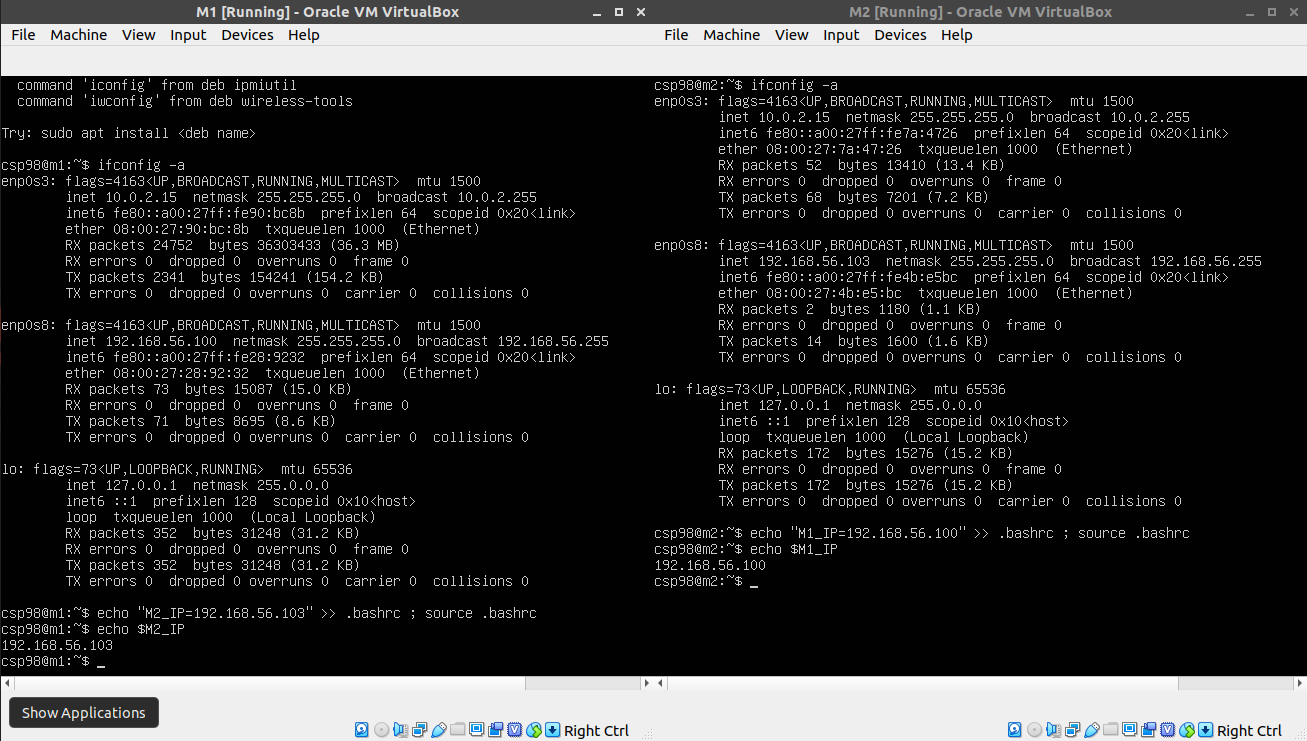
\includegraphics[scale=0.5]{/p1/ip_variable.png}
	\end{figure}
	\begin{figure}[H]
		\centering
		\includegraphics[scale=0.5]{/p1/ssh_ok.png}
	\end{figure}
	\item Creamos en \emph{M2} un documento HTML (\emph{/var/www/html/ejemplo.html}) con el siguiente contenido:
	\begin{lstlisting}
		<HTML>
		<BODY>
		Web de ejemplo de <nombre usuario> para SWAP
		</BODY>
		</HTML>
	\end{lstlisting}
	\item Hacemos \emph{curl} desde la otra máquina y comprobamos que recibimos la respuesta esperada:
	\begin{figure}[H]
		\centering
		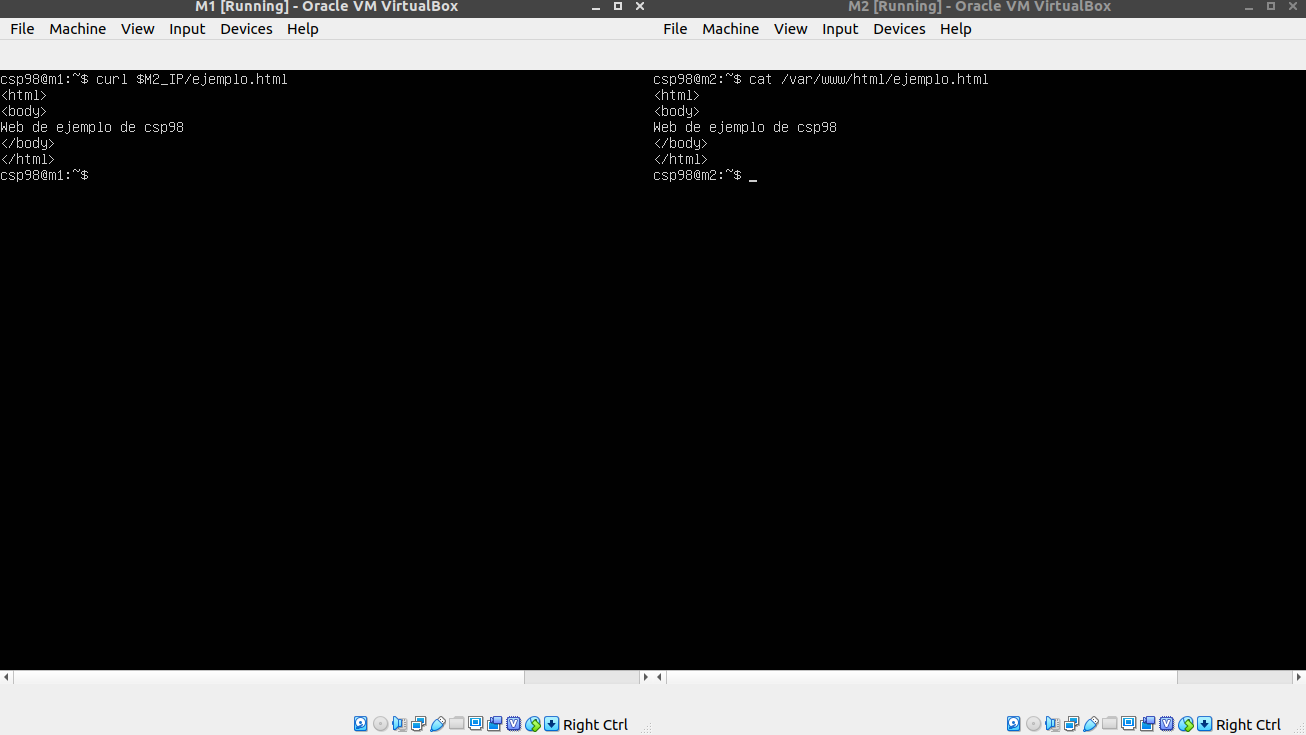
\includegraphics[scale=0.5]{/p1/curl_ok.png}
	\end{figure}
\end{enumerate}

\section{Práctica 2}

En esta práctica clonaremos información entre las máquinas.

\begin{enumerate}
	\item Comenzamos copiando un directorio de m1 a la carpeta de usuario de \emph{m2}:
	\begin{lstlisting}
	m1 > mkdir test ; touch test/file1.txt test/file2.txt
	m1 > scp -r test $M2_IP:~
	\end{lstlisting}
	Ejecutamos \emph{ls -lR} en \emph{M2} para ver el resultado:
	\begin{figure}[H]
		\centering
		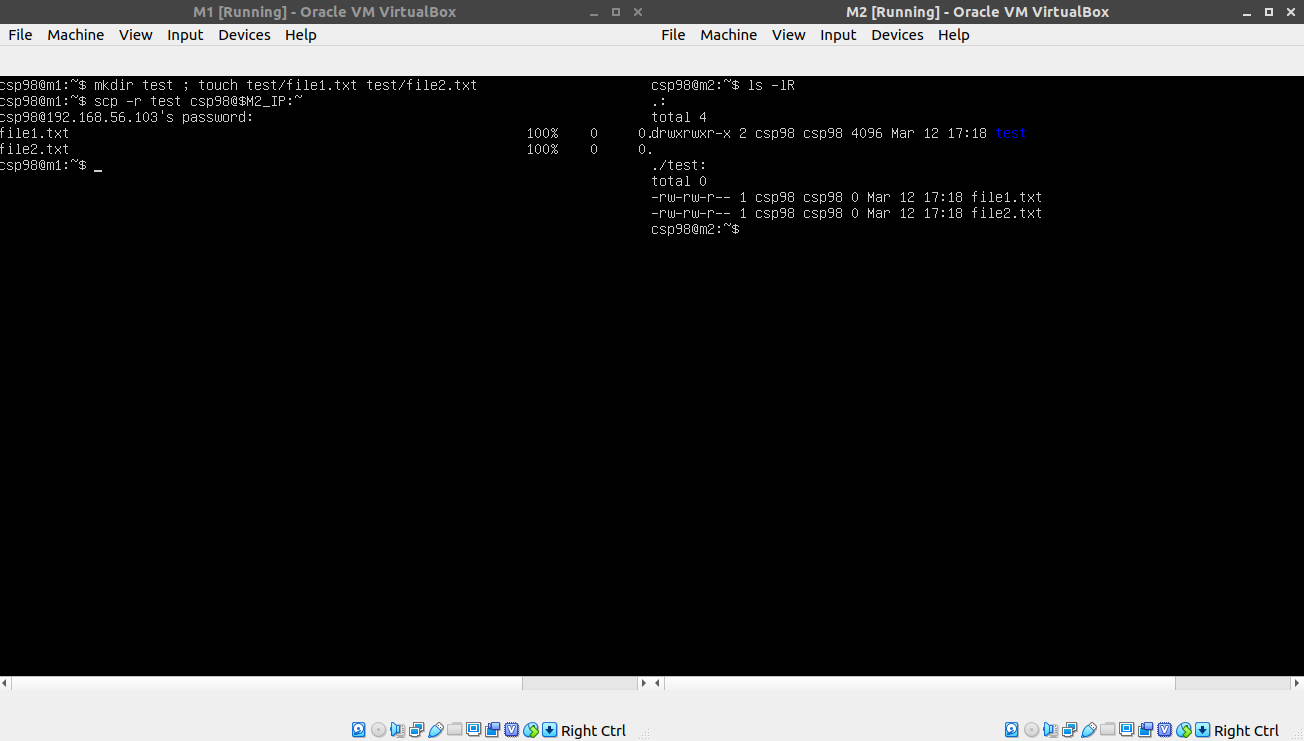
\includegraphics[scale=0.5]{/p2/scp_ok.png}
	\end{figure}
	\item Para no tener que introducir la contraseña en cada conexión SSH configuraremos la autenticación mediante clave público-privada RSA:
	\begin{lstlisting}<HTML>
	m2 > ssh-keygen -b 4096 -t rsa
	\end{lstlisting}
	Pulsamos Enter tres veces.
	\item Copiamos la clave a M1:
	\begin{lstlisting}
	m2 > ssh-copy-id $M1_IP
	\end{lstlisting}
	Introducimos la clave \emph{Swap1234}
	\item Probamos a realizar la conexión. Veremos que no nos pide la clave.
	\begin{figure}[H]
		\centering
		\includegraphics[scale=0.65]{/p2/ssh_ok.png}
	\end{figure}
	\item Por último programamos una tarea de clonación que se ejecutará cada dos horas. De esta forma el contenido de M1 se replicará en M2 cada dos horas. Usaremos \emph{crontab} para ello:
	\item Lo primero que debemos hacer es configurar la clave público privada por ssh en M1 para que no se pida en cada copia (igual que en el paso anterior).
	\item Después damos permisos a nuestro usuario para escribir en el directorio:
	\begin{lstlisting}
	m2 > sudo chown $USER:$USER -R /var/www
	\end{lstlisting}
	\item Instalamos la herramienta \emph{rsync} en M2:
	\begin{lstlisting}
	m2 > sudo apt install -y rsync
	\end{lstlisting}
	\item Configuramos el clonado:
	\begin{lstlisting}
	m2 > sudo nano /etc/crontab
	\end{lstlisting}
	Añadimos la siguiente línea:
	\begin{lstlisting}
	00 */12 * * * csp98 rsync -avz -e ssh 192.168.56.100:/var/www /var/
	\end{lstlisting}
	\item Si queremos probar el funcionamiento del comando podemos establecer una periodicidad menor, crear un archivo en M1 y ver que se replica en M2.
\end{enumerate}
\newpage
\section{Práctica 3}
En esta práctica configuraremos varios balanceadores de carga y los probaremos mediante tests de estrés.
\subsection{Instalación de balanceadores}
\begin{enumerate}
	\item Comenzamos creando una nueva máquina (M3) e instalando Ubuntu Server. Le añadiremos también el adaptador \emph{host-only}.
	\item Almacenamos el alias de ambas IPs para ahorrar tiempo en futuros comandos:
		\begin{lstlisting}
	m3 > echo "M1_IP=192.168.56.100" >> .bashrc ; source .bashrc
	m3 > echo "M2_IP=192.168.56.103" >> .bashrc ; source .bashrc
		\end{lstlisting}
	\item Instalamos nginx y lo lanzamos:
		\begin{lstlisting}
	m3 > sudo apt update ; sudo apt install nginx
	m3 > sudo systemctl start nginx
		\end{lstlisting}
	\item Como solo queremos que funcione como balanceador de carga, desactivamos la funcionalidad de servidor web. Para ello editamos el archivo de configuración y comentamos la siguiente línea:
		\begin{lstlisting}
	m3 > sudo nano /etc/nginx/nginx.conf
		\end{lstlisting}
			\begin{lstlisting}
	# include /etc/nginx/sites-enabled/*
			\end{lstlisting}
		\item Configuramos el \emph{upstream}, máquinas entre las que se dividirá el tráfico:
		\begin{lstlisting}
	m3 > sudo nano /etc/nginx/conf.d/default.conf
		\end{lstlisting}
		Insertamos el siguiente contenido:
		\begin{lstlisting}
	upstream servidoresSWAP{
		server 192.168.56.100;
		server 192.168.56.103;
	}

	server{
		listen 80;
		server_name balanceador;
		access_log /var/log/nginx/balanceador.access.log;
		error_log /var/log/nginx/balanceador.error.log;
		root /var/www/;
		location /
		{
			proxy_pass http://servidoresSWAP;
			proxy_set_header Host $host;
			proxy_set_header X-Real-IP $remote_addr;
			proxy_set_header X-Forwarded-For $proxy_add_x_forwarded_for;
			proxy_http_version 1.1;
			proxy_set_header Connection "";
		}
	}
		\end{lstlisting}
		\item Reiniciamos el servicio para que los cambios surtan efecto:
		\begin{lstlisting}
	m3 > sudo service nginx restart
		\end{lstlisting}
		\item Arrancamos M1 y M2. Para diferenciar a cual de ellas se envía la petición a través del balanceador de carga, modificaremos el archivo \emph{/var/www/html/ejemplo.html} de cada una:
		\begin{figure}[H]
			\centering
			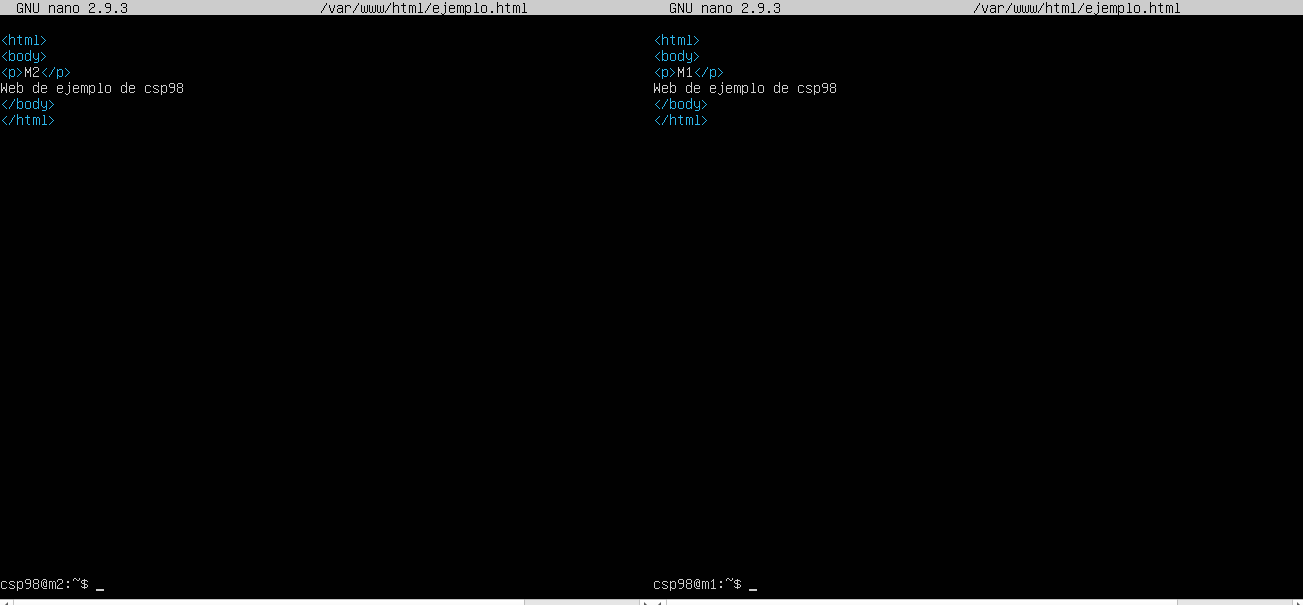
\includegraphics[scale=0.5]{/p3/web_contents.png}
		\end{figure}
		\item Consultamos la IP de M3 y entramos a \emph{192.168.56.104/ejemplo.html} desde el navegador de nuestro host:
		\begin{lstlisting}
	m3 > ip addr | grep 192
		\end{lstlisting}
		\item Recargamos varias veces la página y podremos ver como la petición la atiende un servidor u otro.
		\item Probaremos ahora a repartir la carga de forma desigual. M1 atenderá el doble de peticiones que M2. Para ello editamos el siguiente archivo de configuración y añadimos la directiva \emph{weight}:
		\item Configuramos el \emph{upstream}, máquinas entre las que se dividirá el tráfico:
		\begin{lstlisting}
	m3 > sudo nano /etc/nginx/conf.d/default.conf
		\end{lstlisting}
		\begin{lstlisting}
	upstream servidoresSWAP{
		server 192.168.56.100 weight=2;
		server 192.168.56.103 weight=1;
	}
		\end{lstlisting}
		\item Reiniciamos el servicio y probamos a acceder con el navegador a la IP anterior y refrescar la página.
		\item Tambien podemos especificar políticas para mantener la sesión:
		\begin{itemize}
			\item \textbf{Keep-alive}: las peticiones se enviarán al mismo servidor durante $n$ segundos.
			\begin{lstlisting}
		upstream servidoresSWAP{
			server 192.168.56.100;
			server 192.168.56.103;
			keepalive <n>;
		}
			\end{lstlisting}
			\item \textbf{IP-hash}. Una vez que un servidor atiende una IP, la atenderá siempre. No se recomienda su uso (no se balancea la carga de forma equitativa).
			\begin{lstlisting}
		upstream servidoresSWAP{
			ip_hash;
			server 192.168.56.100;
			server 192.168.56.103;
		}
			\end{lstlisting}
		\end{itemize}
	\item Ahora pasamos a \emph{haproxy}, otro balanceador. Comenzamos instaládolo:
	\begin{lstlisting}
	m3 > sudo apt install -y haproxy
	\end{lstlisting}
	\item Configuramos el balanceador:
	\begin{lstlisting}
	m3 > sudo nano /etc/haproxy/haproxy.cfg
	\end{lstlisting}
	Introducimos las siguientes líneas al final del archivo:
	\begin{lstlisting}
	frontend http-in
		bind *:80
		default_backend servidoresSWAP
	backend servidoresSWAP
		server m1 192.168.56.100:80 maxconn 32
		server m2 192.168.56.103:80 maxconn 32
	\end{lstlisting}
	\item Desactivamos \emph{nginx} y reiniciamos \emph{haproxy}:
	\begin{lstlisting}
	m3 > sudo service nginx stop
	m3 > sudo service haproxy restart
	\end{lstlisting}
	\item Comprobamos su funcionamiento:
	\begin{figure}[H]
		\centering
		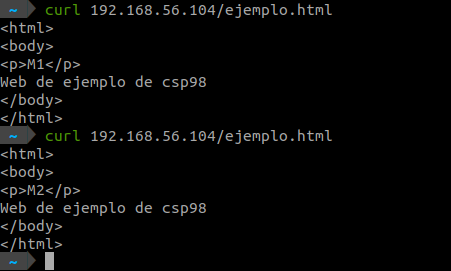
\includegraphics[scale=0.65]{/p3/test_haproxy.png}
	\end{figure}
	\item Por último usaremos un balanceador más, \emph{pen}. Comenzamos instalándolo:
	\begin{lstlisting}
	m3 > sudo apt install -y pen
	\end{lstlisting}
	\item Paramos \emph{haproxy}:
	\begin{lstlisting}
	m3 > sudo service haproxy stop
	\end{lstlisting}
	\item Establecemos el balanceador con el algoritmo round-robin:
	\begin{lstlisting}
	m3 > sudo pen 80 -r $M1_IP:80 $M2_IP:80
	\end{lstlisting}
	\item Comprobamos que funciona:
	\begin{figure}[H]
		\centering
		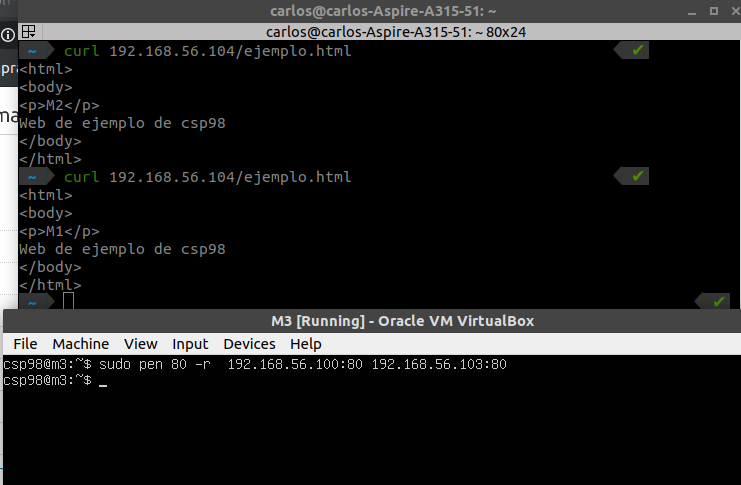
\includegraphics[scale=0.65]{/p3/pen_ok.png}
	\end{figure}
\end{enumerate}
\subsection{Test de rendimiento en balanceadores mediante \emph{ab}}
En esta sección someteremos los distintos balanceadores a una carga alta mediante \emph{Apache Benchmark} y mediremos su rendimiento en función del tiempo de respuesta obtenido.
\begin{enumerate}
	\item Comenzamos instalando la utilidad en nuestro host:
	\begin{lstlisting}
	host > sudo apt install -y apache2-utils
	\end{lstlisting}
	\item Ejecutamos el siguiente test contra los distintos balanceadores:
	\begin{lstlisting}
	host > ab -n 10000 -c 10 http://192.168.56.104/ejemplo.html
	\end{lstlisting}
\end{enumerate}
Los tiempos medios de respuesta obtenidos tras realizar tres ejecuciones y calcular la media aritmética fueron los siguientes:
\begin{figure}[H]
	\centering
	\begin{tabular}{|c|c|}
		\hline
		\textbf{Balanceador} & \textbf{Tiempo de respuesta por petición (ms)} \\
		\hline
		\emph{haproxy} & 5.054 \\
		\hline
		\emph{nginx} & 6.458 \\
		\hline
		\emph{pen} & 5.353 \\
		\hline
	\end{tabular}
\end{figure}
En este caso concluimos con que \emph{haproxy} ofrece mejor rendimiento que \emph{nginx} y \emph{pen}.

\section{Práctica 4}

En esta práctica configuraremos la seguridad de nuestra granfa mediante un certificado y un cortafuegos.

\subsection{Creación del certificado autofirmado para acceder por HTTPS}

\begin{enumerate}
	\item Comenzamos activando el módulo SSL de Apache en M1:
	\begin{lstlisting}
	m1 > sudo a2enmod ssl; sudo service apache2 restart
	\end{lstlisting}
	\item Creamos el certificado:
	\begin{lstlisting}
	m1 > sudo mkdir /etc/apache2/ssl
	m1 > sudo openssl req -x509 -nodes -days 365 -newkey rsa:2048 -keyout /etc/apache2/ssl/apache.key -out /etc/apache2/ssl/apache.crt
	\end{lstlisting}
	\item Configuramos los siguientes datos:
		\begin{itemize}
			\item \textbf{Country name}: ES.
			\item \textbf{Province name}: Granada.
			\item \textbf{Locality name}: Granada.
			\item \textbf{Organization name}: SWAP.
			\item \textbf{Organizational unit name}: P4.
			\item \textbf{Common name}: nuestro usuario UGR.
			\item \textbf{Email address}: nuestro email UGR.
		\end{itemize}
	\item Ahora utilizaremos ese certificado en M1. Para ello, debemos editar la configuración de nuestro servidor web y especificar la ruta de los certificados:
	\begin{lstlisting}
	m1 > sudo nano /etc/apache2/sites-available/default-ssl.conf
	\end{lstlisting}
	Sustituimos las siguientes líneas bajo \emph{SSLEngine on}:
	\begin{lstlisting}
	SSLCertificateFile /etc/apache2/ssl/apache.crt
	SSLCertificateKeyFile /etc/apache2/ssl/apache.key
	\end{lstlisting}
	\item Activamos el sitio default-ssl y reiniciamos apache:
	\begin{lstlisting}
	m1 > sudo a2ensite default-ssl
	m1 > sudo service apache2 restart
	\end{lstlisting}
	\item Accedemos desde el host a \emph{https://IP M1} y obtenemos la información del certificado:
	\begin{figure}[H]
		\centering
		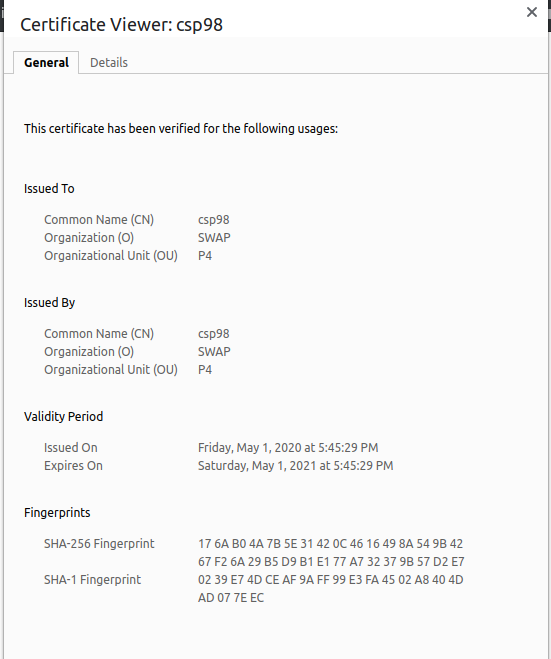
\includegraphics[width=0.5\textwidth]{p4/cert.png}
	\end{figure}
	\item Ahora configuraremos la granja para que funciones bajo SSL. Comenzamos copiando el certificado y la clave a M2 y M3:
	\begin{lstlisting}
	m1 > sudo scp /etc/apache2/ssl/apache.crt <nombre_usuario>@<IP M2>:/home/<nombre_usuario>/apache.crt
	m1 > sudo scp /etc/apache2/ssl/apache.crt <nombre_usuario>@<IP M2>:/home/<nombre_usuario>/apache.key

	m1 > sudo scp /etc/apache2/ssl/apache.crt <nombre_usuario>@<IP M3>:/home/<nombre_usuario>/apache.crt
	m1 > sudo scp /etc/apache2/ssl/apache.crt <nombre_usuario>@<IP M3>:/home/<nombre_usuario>/apache.key
	\end{lstlisting}
	\item Movemos los archivos de certificado a \emph{/etc/apache2/ssl} y realizamos los pasos anteriores en M2.
	\item Creamos un nuevo server en nginx (M3):
	\begin{lstlisting}
	m1 > sudo nano /etc/nginx/conf.d/default.conf
	\end{lstlisting}
	Copiamos las líneas que introdujimos en la práctica anterior, cambiamos \emph{listen 80} por \emph{listen 443 ssl} y añadimos lo siguiente:
	\begin{lstlisting}
	ssl on;
	ssl_certificate /home/<nombre_usuario>/apache.crt;
	ssl_certificate_key /home/<nombre_usuario>/apache.key;
	\end{lstlisting}
	\item Reiniciamos el servicio:
	\begin{lstlisting}
	m1 > sudo systemctl restart nginx
	\end{lstlisting}
	\item Comprobamos desde el navegador que ya podemos hacer peticiones HTTPS.
\end{enumerate}
\subsection{Configuración del cortafuegos}
	\begin{enumerate}
	\item Ahora configuraremos un cortafuegos para que a M1 y M2 solo se pueda acceder desde el balanceador. Para ello elaboraremos un script:
	\begin{lstlisting}
	#!/bin/bash
	# Run this script with superuser permissions!
	# Eliminamos las reglas existentes
	iptables -F;
	iptables -X;
	iptables -Z;
	iptables -t nat -F;
	# Denegamos todo el trafico entrante (politica inicial)
	iptables -P INPUT DROP;
	iptables -P OUTPUT ACCEPT;
	iptables -P FORWARD DROP;
	# Permitir acceso desde las loopback addresses (localhost)
	iptables -A INPUT -i lo -j ACCEPT
	iptables -A OUTPUT -o lo -j ACCEPT
	# Puertos 22 (SSH), 80 (HTTP) y 443 (HTTPS) desde el balanceador
	iptables -A INPUT -s 192.168.56.104 -p tcp -m multiport --dports 22,80,443 -j ACCEPT
	iptables -A INPUT -s 192.168.56.104 -p tcp -m multiport --sports 22,80,443 -j ACCEPT
	\end{lstlisting}
	\item Hacemos que el script se ejecute al inicio del sistema:
	\begin{lstlisting}
	m1, m2 > sudo crontab -e
	\end{lstlisting}
	Añadimos lo siguiente al final:
	\begin{lstlisting}
	@reboot sudo /home/<nombre_usuario>/iptables_servers.sh
	\end{lstlisting}
	\item Finalmente creamos un script para M3 (sólo aceptará peticiones HTTP y HTTPS):
	\begin{lstlisting}
	#!/bin/bash
	# Run this script with superuser permissions!
	# Eliminamos las reglas existentes
	iptables -F;
	iptables -X;
	iptables -Z;
	iptables -t nat -F;
	# Denegamos todo el trafico entrante (politica inicial)
	iptables -P INPUT DROP;
	iptables -P OUTPUT ACCEPT;
	iptables -P FORWARD DROP;
	# Permitir acceso desde las loopback addresses (localhost)
	iptables -A INPUT -i lo -j ACCEPT
	iptables -A OUTPUT -o lo -j ACCEPT
	# Puertos 80 (HTTP) y 443 (HTTPS) desde cualquier IP
	iptables -A INPUT -p tcp -m multiport --dports 80,443 -j ACCEPT
	iptables -A INPUT -p tcp -m multiport --sports 80,443 -j ACCEPT
	\end{lstlisting}
	\item Repetimos el procedimiento anterior en M3 para que se ejecute el script al inicio.
\end{enumerate}
\newpage
\section{Práctica 5}
En esta práctica configuraremos la réplica entre bases de datos MySQL en M1 y M2.

\subsection{Clonado manual}
\begin{enumerate}
	\item Comenzamos creando una tabla en M1 e insertando algunos datos:
	\begin{lstlisting}
	m1 > sudo mysql -u root -p
	\end{lstlisting}
	Introducimos nuestra clave, \emph{Swap1234} e insertamos los datos:
	\begin{lstlisting}
	mysql (m1) > CREATE DATABASE estudiante;
	mysql (m1) > USE estudiante;
	mysql (m1) > CREATE TABLE datos(nombre VARCHAR(100), apellidos VARCHAR(100), usuario VARCHAR(100), email VARCHAR(100));
	mysql (m1) > INSERT INTO datos(nombre, apellidos, usuario, email) VALUES ('<nombre>', '<apellidos>', '<usuario UGR>', '<correo UGR>');
	\end{lstlisting}
	Ejecutamos \emph{SELECT * FROM datos;} y deberíamos ver lo siguiente:
	\begin{figure}[H]
		\centering
		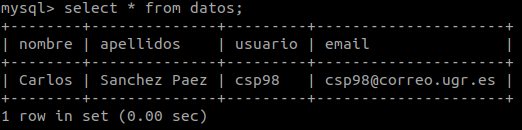
\includegraphics[width=0.65\textwidth]{/p5/select_datos.png}
	\end{figure}
	\item Ahora haremos un backup de la base de datos para replicarla en M2. Primero tendremos que bloquear las tablas para que no se escriba en ellas:
	\begin{lstlisting}
	mysql (m1) > FLUSH TABLES WITH READ LOCK;
	mysql (m1) > exit;
	\end{lstlisting}
	\item Ahora hacemos el backup:
	\begin{lstlisting}
	m1 > sudo mysqldump estudiante -u root -p > /tmp/estudiante.sql
	\end{lstlisting}
	\item Desbloqueamos las tablas:
	\begin{lstlisting}
	m1 > sudo mysql -u root -p
	mysql (m1) > UNLOCK TABLES;
	\end{lstlisting}
	\item Copiamos el backup a M2:
	\begin{lstlisting}
	m1 > sudo scp /tmp/estudiante.sql <usuario>@<IP M2>:/tmp/estudiante.sql
	\end{lstlisting}
	\item Creamos la base de datos en M2 y restauramos el archivo:
	\begin{lstlisting}
	m2 > sudo mysql -u root -p
	mysql (m2) > CREATE DATABASE estudiante;
	mysql (m2) > exit;
	m2 > sudo mysql -u root -p estudiante < /tmp/estudiante.sql
	\end{lstlisting}
\end{enumerate}
\subsection{Configuración maestro-esclavo}
\begin{enumerate}
	\item Editamos el archivo de configuración en M1:
	\begin{lstlisting}
	m1 > sudo nano /etc/mysql/mysql.conf.d/mysqld.conf
	\end{lstlisting}
		\begin{itemize}
			\item Comentamos la línea \emph{bind-address}.
			\item Añadimos los siguientes parámetros:
			\begin{lstlisting}
	log_error = /var/log/mysql/error.log
	server-id = 1
	log_bin = /var/log/mysql/bin.log
			\end{lstlisting}
		\end{itemize}
	\item Reiniciamos el servicio:
	\begin{lstlisting}
	m1 > sudo service mysql restart
	\end{lstlisting}
	\item Pasamos a la configuración del esclavo (M2). Debemos editar el archivo de configuración igual que en M1, pero estableciendo \emph{server-id = 2}.
	\item Crearemos en M1 un usuario para el esclavo, con los permisos necesarios para hacer las réplicas:
	\begin{lstlisting}
	m1 > sudo mysql -u root -p
	mysql (m1) > CREATE USER esclavo IDENTIFIED BY 'esclavo';
	mysql (m1) > GRANT REPLICATION SLAVE ON *.* TO 'esclavo'@'%' IDENTIFIED BY 'esclavo';
	mysql (m1) > FLUSH PRIVILEGES;
	mysql (m1) > FLUSH TABLES;
	mysql (m1) > FLUSH TABLES WITH READ LOCK;
	mysql (m1) > SHOW MASTER STATUS;
	\end{lstlisting}
	Deberíamos ver algo de este estilo:
	\begin{figure}[H]
		\centering
		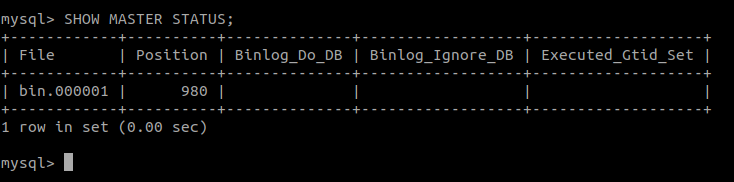
\includegraphics[width=0.65\textwidth]{/p5/master_status.png}
	\end{figure}
	\item Ahora configuraremos el esclavo con los datos obtenidos anteriormente:
	\begin{lstlisting}
	m2 > sudo mysql -u root -p
	mysql (m2) > CHANGE MASTER TO MASTER_HOST='<IP M1>', MASTER_USER='esclavo', MASTER_PASSWORD='esclavo', MASTER_LOG_FILE='bin.000001', MASTER_LOG_POS=980, MASTER_PORT=3306;
	mysql (m2) > exit;
	\end{lstlisting}
	\item Desactivamos el firewall en las máquinas:
	\begin{lstlisting}
	m1, m2 > sudo iptables -A OUTPUT -j ACCEPT ; sudo iptables -A INPUT -j ACCEPT
	\end{lstlisting}
	\item Arrancamos el esclavo en M2, desbloqueamos tablas en M1 y vemos el estado del esclavo:
	\begin{lstlisting}
		mysql (m2) > START SLAVE;
		mysql (m1) > UNLOCK TABLES;
		mysql (m2) > SHOW SLAVE STATUS\G
	\end{lstlisting}
	\begin{figure}[H]
		\centering
		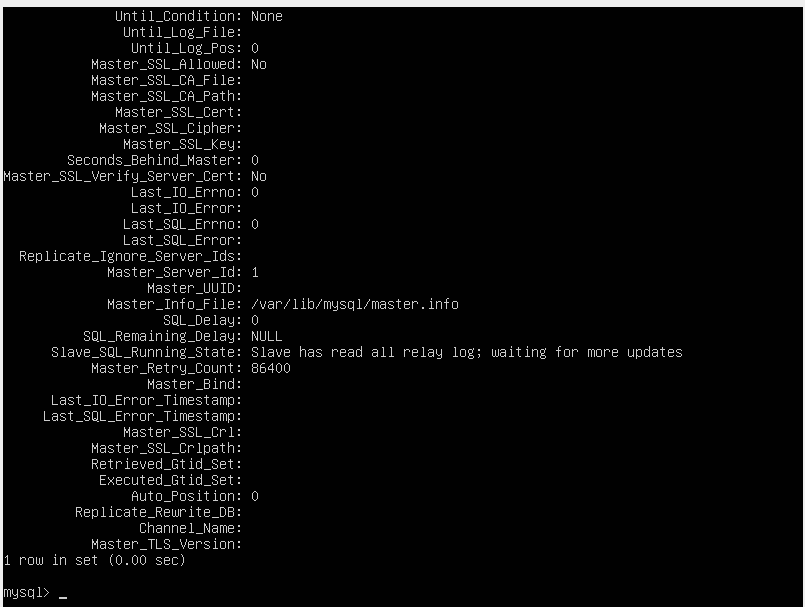
\includegraphics[width=0.65\textwidth]{/p5/slave_status.png}
	\end{figure}
	Deberíamos tener el parámetro \emph{SECONDS\_BEHIND\_MASTER} a un valor distinto de NULL.
	\item Creamos una entrada en M1 y vemos como se replica en M2:
	\begin{lstlisting}
	mysql (m1) > USE estudiante;
	mysql (m1) > INSERT INTO datos VALUES("test12", "test", "test", "test");
	\end{lstlisting}
	\begin{figure}[H]
		\centering
		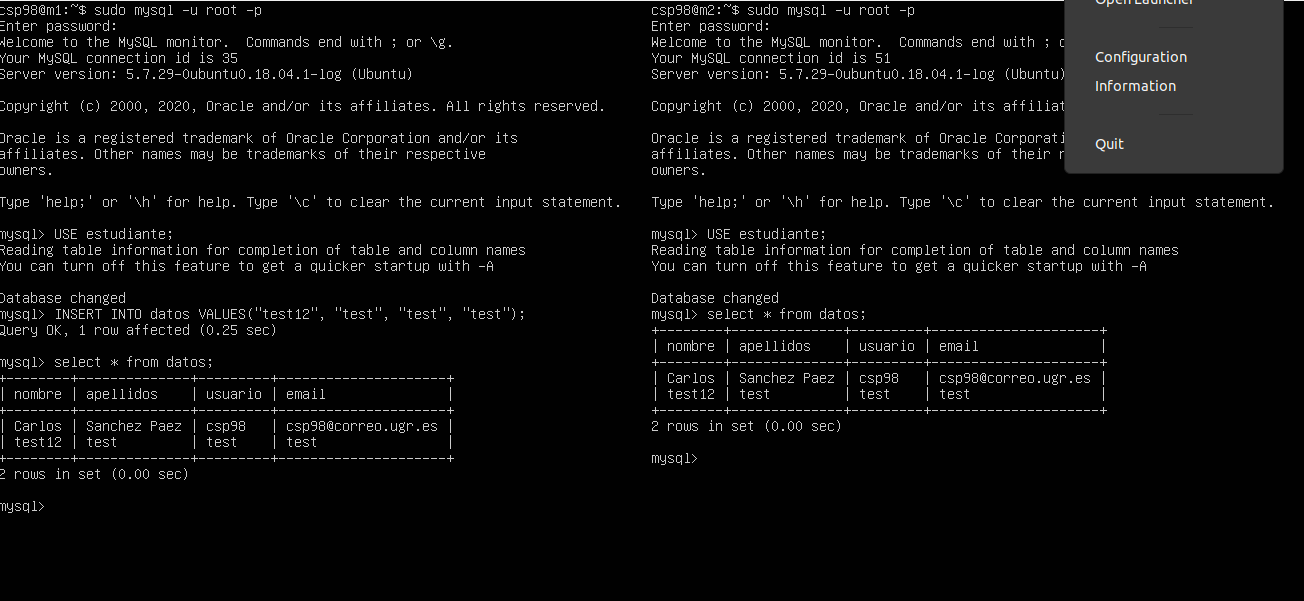
\includegraphics[width=0.65\textwidth]{/p5/value_replication.png}
	\end{figure}
\end{enumerate}
\subsection{Configuración maestro-maestro}
\begin{enumerate}
	\item Comenzamos creando el usuario esclavo en M2 y dándole permisos:
	\begin{lstlisting}
	mysql (m2) > CREATE USER esclavo2 IDENTIFIED BY 'esclavo2';
	mysql (m2) > GRANT REPLICATION SLAVE ON *.* TO 'esclavo2'@'%' IDENTIFIED BY 'esclavo2';
	mysql (m2) > FLUSH PRIVILEGES;
	mysql (m2) > FLUSH TABLES;
	mysql (m2) > FLUSH TABLES WITH READ LOCK;
	mysql (m2) > SHOW MASTER STATUS;
	\end{lstlisting}
	\item Configuramos M1 con los datos obtenidos:
	\begin{lstlisting}
	mysql (m1) > CHANGE MASTER TO MASTER_HOST='<IP M2>', MASTER_USER='esclavo2', MASTER_PASSWORD='esclavo2', MASTER_LOG_FILE=<valor File>, MASTER_LOG_POS=<valor Position>, MASTER_PORT=3306;
	\end{lstlisting}
	\item Arrancamos el esclavo y desbloqueamos las tablas en el maestro:
	\begin{lstlisting}
		mysql (m1) > START SLAVE;
		mysql (m2) > UNLOCK TABLES;
		mysql (m1) > SHOW SLAVE STATUS\G
	\end{lstlisting}
	\item Insertamos valores para asegurarnos de que funciona bien:
	\begin{figure}[H]
		\centering
		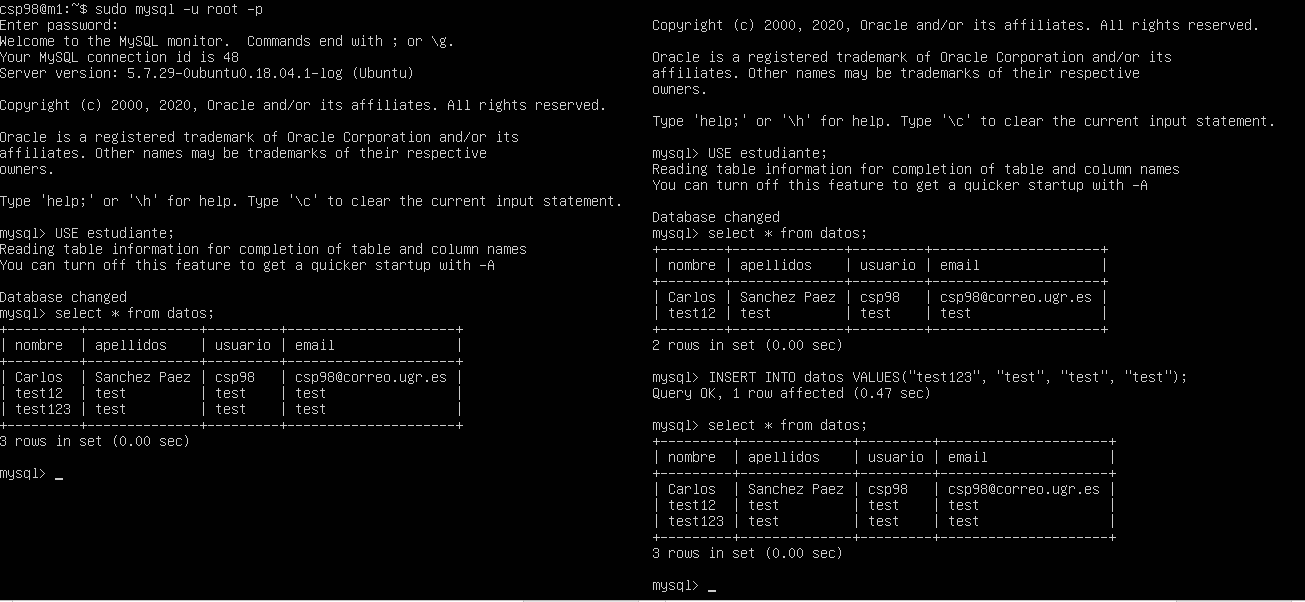
\includegraphics[width=0.65\textwidth]{/p5/master_master_replication.png}
	\end{figure}
\end{enumerate}






\end{document}
